\documentclass{article}
\usepackage[utf8]{inputenc}
\usepackage[T1]{fontenc}
\usepackage{graphicx}
\usepackage{hyperref}
\usepackage{geometry}
\geometry{margin=1in}

\title{BYLAWS}
\date{Encyclopaedia Britannica (1771)}

\begin{document}
\maketitle

\section*{Historical source}
\textbf{Entry ID:} \texttt{entry-bylaws-2250} \\
\textbf{Volume ID:} 144133901 \\
\textbf{Character Count:} 316

\subsection*{Extracted Text}
BYLAWS, or ByrŁLAWS, private and peculiar laws for the good government of a city, court, or other community, made by the general content of the mem-bers.

All by-laws are to be reafonable, and for the com-mon benefit, not private advantage of any particular prefers, and mult be agreeable to the public laws in bang.



\section*{Source record}
\begin{itemize}
\item \textbf{Dataset:} \texttt{NationalLibraryOfScotland/encyclopaedia\_britannica\_illustrated}
\item \textbf{Dataset Revision:} \texttt{309f765b1ecc83e0a7f7762e44b4a927a7555443}
\item \textbf{Page ID:} \texttt{britannica:309f765b1ecc83e0a7f7762e44b4a927a7555443:train:2250} \\
  \textbf{Filename:} \texttt{page-2250-75315f455009.jpg} \\
  \textbf{Row Index:} 2250 \\
  \textbf{SHA256:} \texttt{75315f45500988da...}
\end{itemize}

\begin{figure}[h]
\centering
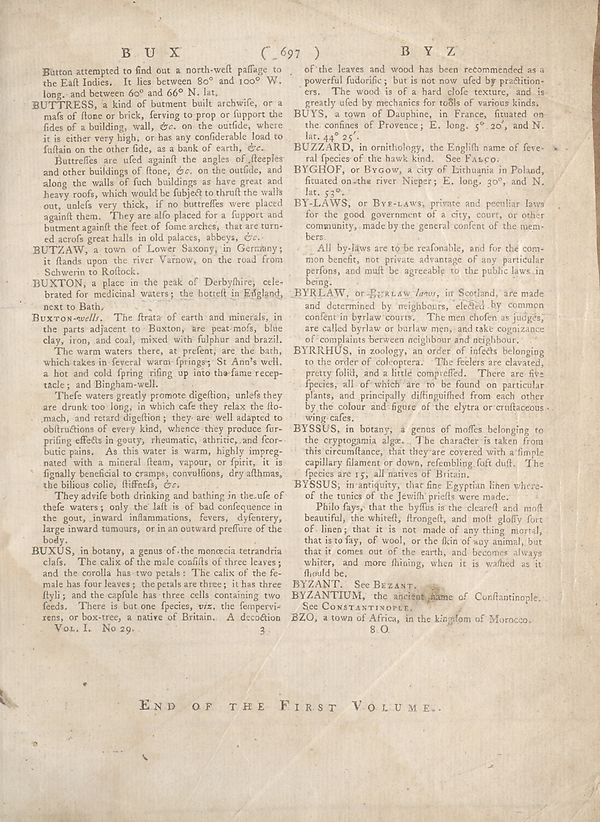
\includegraphics[width=0.85\textwidth]{../scans/page-2250-75315f455009.jpg}
\caption*{Source scan: \texttt{page-2250-75315f455009.jpg}}
\end{figure}

\end{document}
